\chapter{Controller Design}\label{chap:Control}
Attitude controller: Statespace 
Translational controller: X and Y two p controlles in cascade 
clasical controller, bodeplots, root locus. 


The system of the quadcopter has been described by a mathematical model, that is to be used in the design of a control system. The control system must stabilize the naturally unstable system of the quadcopter. It shall also ensure the desired behaviour, that is a stable flying mode, that can tolerate distubances \fxnote{we have not said that, purhaps, the text should just be removed.}

\section{Design Considerations}
What do we want from the design of controller? \\
Steady state error: \\
Rise time: \\
Settling time:\\
Overshoot:\\
Phase margin: \\
Gain margin: \\
These must be set in a chapter after system description, where requirements are set and reasoned. \\
\\

The model consists of two submodels, an attitude model and a translational model. It is therefore desirable to design two control systems, one for each model. These will however have to interact, as they share input and rely on each other. 

\begin{figure}[H]
	\centering
	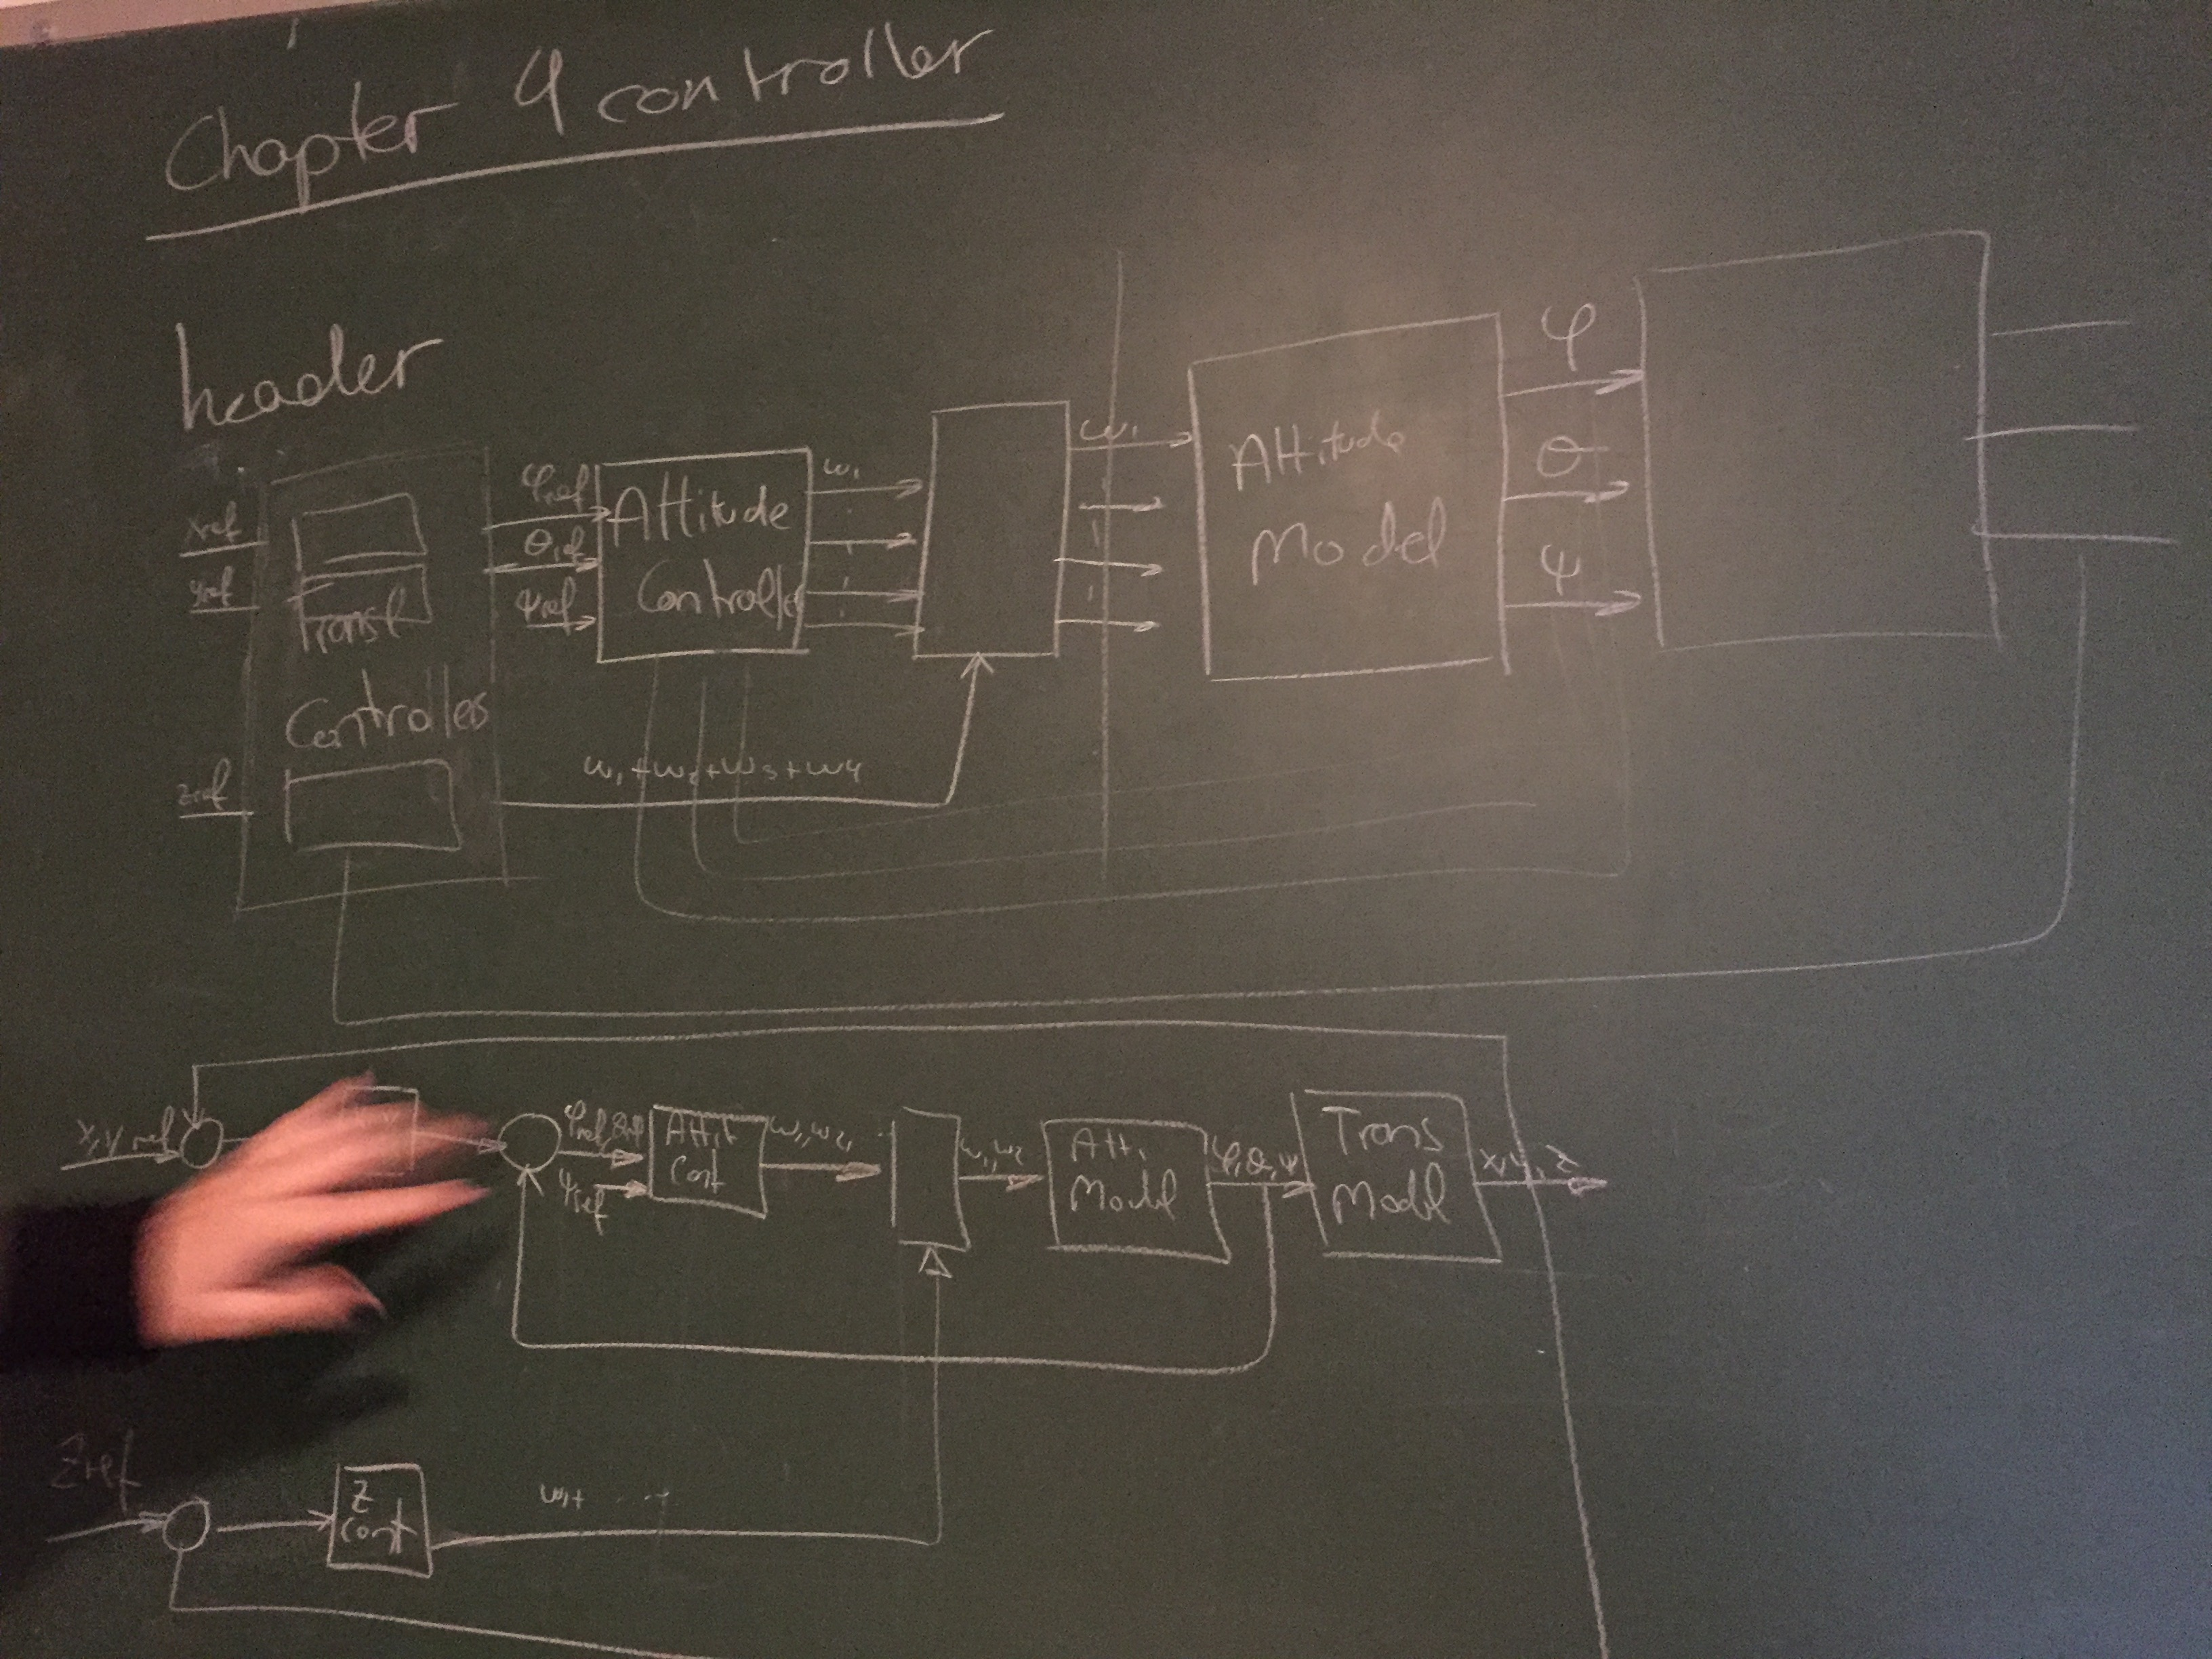
\includegraphics[width=0.7 \textwidth]{figures/ControlHeadDiagram.JPG}
	\caption{Block diagram of overall control system.}
	\label{fig:ControlHeadDiagram}
\end{figure}


\autoref{fig:ControlHeadDiagram} is a block diagram of the overall control system.
The attitude controller is an inner controller and is designed as state space, as this allows multiple inputs. The three angles roll, pitch and yaw are coupled and therefore complex to control individually, as the single controllers will disturb each other resulting in a less effective control system. The translational control system is going to be classical control, where bode plots and root locus are the design method to obtain proportional controllers. 

First the design of the attitude controller is done followed by the design of the translational controller. 
When the controllers are designed, they are simulated with the linear models to ensure, that the desired behaviour is obtained by the obtained designs. Afterwards the controllers are simulated with the models, that are not linearized, as these represent the true behaviour of the system. If the controllers yield an acceptable outcome, they are to be implemented in the system. To do so, they are first discretized. It is nesecary to simulate the discrete controllers and compare the results with the continuous controllers, as some design considerations may be lost in the dicretization. Lastly the controllers are implemented on the micro controller and the system is to be tested in the Vicon room. 

